\chapter{Dimensionality reduction (time-series decomposition) and indexing.}
The problem addressed in this chapter is the approximation (lossy compression) of a time series data in a way which allows to maintain a fast random access, comparison and indexing of the time-series with minimal errors. There are many approximation proposed in the research literature and the Figure \ref{fig:approximations} from \cite{citeulike:2821475} illustrates their hierarchy.

All of the methods essentially aiming to overcome the problem of the high-dimensionality of the time series data in order to utilize data-mining, indexing and clustering algorithms. 


\begin{figure}[tbp]
   \centering
   \includegraphics[height=45mm]{ts_representations.eps}
   %%{seriesheatmap}
   \caption{The figure from \cite{citeulike:2821475} illustrating a hierarchy of all the various time series representations.}
   \label{fig:approximations}
\end{figure} 
